%!TEX root = ../thesis.tex
%Adding the above line, with the name of your base .tex file (in this case "thesis.tex") will allow you to compile the whole thesis even when working inside one of the chapter tex files
\chapter{Coronal Mass Ejection and Plasma Shock Theory} 
\label{chap:2}

\section{Plasma Physics and Magnetohydrodynamics}\label{sec:1}

\subsection{Maxwell's Equations}\label{sec:10}

\subsection{Plasma Physics and Boltzmann Equation}\label{sec:11}

\subsection{Magnetohydrodynamics}\label{sec:12}

\subsection{Magnetic Reconnection}\label{sec:13}

\subsection{MHD Rankine-Hugoniot Equations}\label{sec:14}

\subsection{Bow Shocks}\label{sec:15}



\section{Coronal Mass Ejections}\label{sec:2}

\subsection{Catastrophe Model}\label{sec:20}

\subsection{Magnetic Breakout Model}\label{sec:21}

\subsection{Toroidal Instability}\label{sec:22}

\subsection{Drag Models}\label{sec:23}


\section{Coronal Shocks and Plasma Emission}\label{sec:3}

\subsection{Shock Particle Acceleration}\label{sec:30}

\subsection{Wave-Particle Interaction}\label{sec:31}

Quasi-linear relaxation
\begin{figure}[!t]
\begin{center}
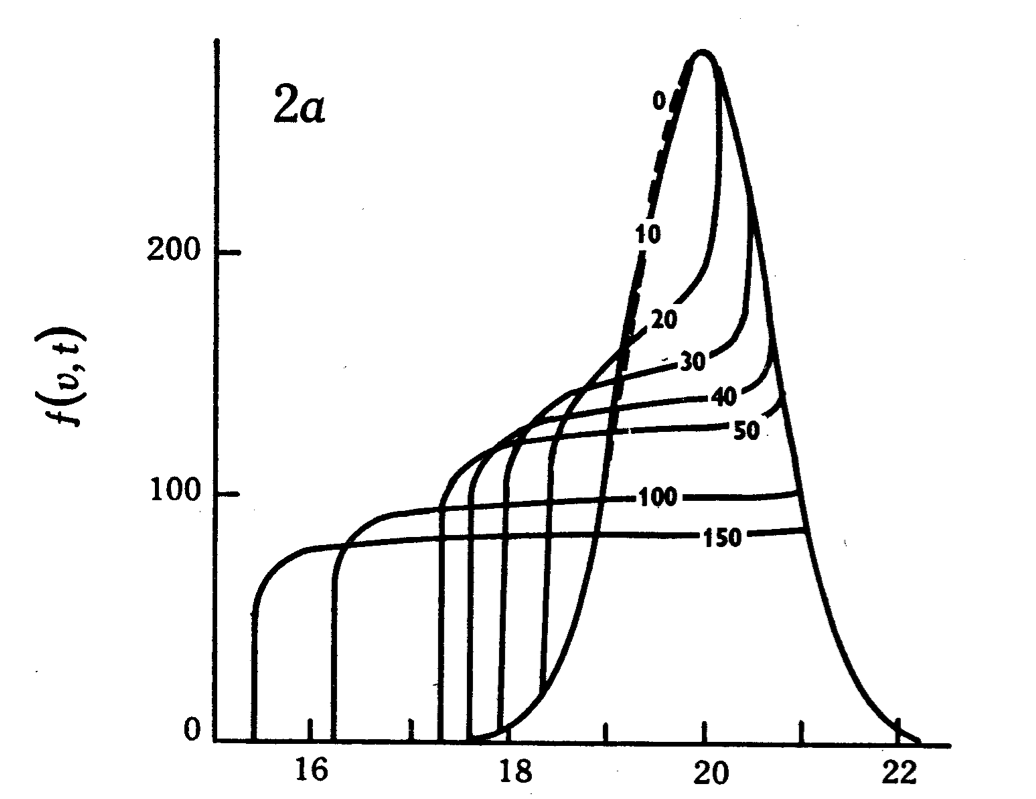
\includegraphics[scale=0.35, trim = 4cm 0cm 0cm 0cm]{images/Grognard1975}
\end{center}
\end{figure}


\subsection{Three-Wave Interaction and Plasma Emission}\label{sec:32}

Once the Langmuir waves are produced from the bump-on-tail instability a number of wave interaction processes occur in order to bring about plasma emission. This involves the interaction of various wave modes in the plasma described by a mathematical formalism called the three-wave interaction. In this process three wave modes in a plasma M, P, and Q are described by their distribution functions in a wave-number space ($k$-space). the distribution functions are given by $N_M(k_M)$, $N_P(k_P)$, $N_Q(k_Q)$, where the $N$ describe the occupation number of wave quanta between $k$ and $k+dk$ in the wave-number space. Waves in P and Q mode may interact to such that wave quanta are removed from the P and Q k-space and added to the M k-space. This is essentially an emission of an energy packet from the P and Q -space to the M k-space. The rate of change of occupation numbers in the three k-spaces are given by
\begin{equation}
\frac{dN_M(\mathbf{k}_M)}{dt} = -\int \frac{d^3\mathbf{k}_P}{(2\pi)^3}\int \frac{d^3\mathbf{k}_Q}{(2\pi)^3}g(\mathbf{k}_M, \mathbf{k}_P, \mathbf{k}_Q)
\end{equation}
\begin{equation}
\frac{dN_P(\mathbf{k}_P)}{dt} = -\int \frac{d^3\mathbf{k}_M}{(2\pi)^3}\int \frac{d^3\mathbf{k}_Q}{(2\pi)^3}g(\mathbf{k}_M, \mathbf{k}_P, \mathbf{k}_Q)
\end{equation}
\begin{equation}
\frac{dN_Q(\mathbf{k}_Q)}{dt} = -\int \frac{d^3\mathbf{k}_M}{(2\pi)^3}\int \frac{d^3\mathbf{k}_P}{(2\pi)^3}g(\mathbf{k}_M, \mathbf{k}_P, \mathbf{k}_Q)
\end{equation}
where $g(\bf{k}_M, \bf{k}_P, \bf{k}_Q)$ is incorporates a transition probability for wave quanta into and out of energy states in the various k-spaces \citep{robinson1994}. The transition probability is given by
\begin{multline}
g(\mathbf{k}_M, \mathbf{k}_P, \mathbf{k}_Q) = u_{MPQ}(\mathbf{k}_M, \mathbf{k}_P, \mathbf{k}_Q)   [N_M(\mathbf{k_M}) N_P(\mathbf{k_P})  - \\ 
N_P(\mathbf{k_P}) N_Q(\mathbf{k_Q})   +N_Q(\mathbf{k_Q}) N_M(\mathbf{k_M})  ]
\end{multline}
where $u_{MPQ}(\bf{k}_M, \bf{k}_P, \bf{k}_Q) $ is the transition probability from states in P and Q  to M, for example \citep{melrose1986}. $u_{MPQ}$ is analogous to transition probabilities given by the Einstein coefficients for transferring energy packets from and atomic state to a photon state (photon emission) i.e., whereas the Einstein coefficients are used in atom-wave (atom-photon) energy exchanges, $u_{MPQ}$ describes wave-wave energy exchanges. The transition probability is given by
\begin{equation}
u_{MPQ}(\mathbf{k}_M, \mathbf{k}_P, \mathbf{k}_Q)  \propto \delta(\omega_M - \omega_P - \omega_Q ) \delta^3(\mathbf{k}_M - \mathbf{k}_P - \mathbf{k}_Q )
\end{equation}
where the $\omega$ are the frequency of the corresponding wave and and $\delta$ are delta functions. Given the presence of delta functions in the transition probability expression, we can see that an exchange of energy quanta amongst the wave modes can only occur when 
\begin{eqnarray}
\omega_M & = & \omega_P + \omega_Q \\
\mathbf{k}_M & = & \mathbf{k}_P + \mathbf{k}_Q
\end{eqnarray}

Hence for an a conversion wave modes in a plasma such as $M \rightarrow P + Q$ (a decay of mode M into P and Q), or it's reverse process $P + Q \rightarrow M $ (a coupling of P and Q to produce M) is described by equations (2.1) to (2.7). 

The production of plasma emission after a bump-on-tail instability has occurred requires a three wave interaction amongst a Langmuir wave $L$, ion acoustic wave $S$, and electromagnetic wave $T$. Fundamental emission during a radio burst occurs via a decay of Langmuir waves into an electromagnetic and ion sound wave
\begin{equation}
L \rightarrow T + S
\end{equation}
while second harmonic first requires the decay $L\rightarrow L^{'} + S$, where $L^{'}$ is a product Langmuir wave propagating in the opposite direction to the first. This is followed by a coalescence of the original and product Langmuir waves
\begin{equation}
L + L^{'}\rightarrow T'
\end{equation}


\begin{itemize}
\item The dispersion relations
\item Source emissivities
\end{itemize}











